% Results and discussion

\chapter{Results and Discussion} \label{ch:res_and_disc}

This chapter describes the obstacles and insights what have been faced during the implementation of the project and how the results came out to be.
It gives variations of what could have done differently and how the project can be improved in the future.
The chapter also discusses the pros and cons about the current maintainability.

\section{Results}
The implementation of this project offers a script that automates the process of adding new applications with new devices to a ChirpStacks server from an Excel file, with addition to add devices to an application that is already on the server and listed in the Excel file.
It also provides a possibility to delete single devices from the chosen application, as well as a possibility to delete an application with its devices from the server.

The implementation fulfills all of the requirements that were set in the beginning of the project with the additional request for a feature to delete an application by using its name.
The end result provides the user a way to handle the tasks more effectively than previously by reducing the possible human errors in writing and by speeding up the process.
As the implementation can be executed repeatedly, when the settings and other factors are still the same, it can potentially save a lot of time from the educators.

The effectiveness of the implementation has been tested by comparing the workload of adding a new application with a set of devices to the server either manually or by using the implementation.
The testing also took in consideration about the difference if the browser is run headless or with the visible window.
The manual part was implemented by using the same Excel file where the details where added, and that was applied by writing all the details fully manually and by using the copy-paste method to speed things up a bit.
The test is only done by one person, therefore the writing speed is a changing factor and the time measuring is not as specific, as it would be if the time would be measured by an other person, or a computer.

Below there are three plots shown. Each one represents one test case. First one is to create an application with 5 devices in Figure\ref{fig:5_devices}, second with 20 devices in Figure\ref{fig:20_devices} and third with 45 devices in Figure\ref{fig:45_devices}.
The time that has been used to select the command to create the application and then the wanted application is excluded from the time measurements.

Each plot shows the amount of time it has taken to add the devices to the application by executing it in three different ways, manually, using the windowed mode and the headless mode of the implementation.
Time is an increasing curve showing the total amount used in the process of adding the devices.
Three tables are attached to Appendix~\ref{appx:tables}to show the amount of time to create application in the same three methods that are used in the plotting.

\begin{figure}[H]
\centering
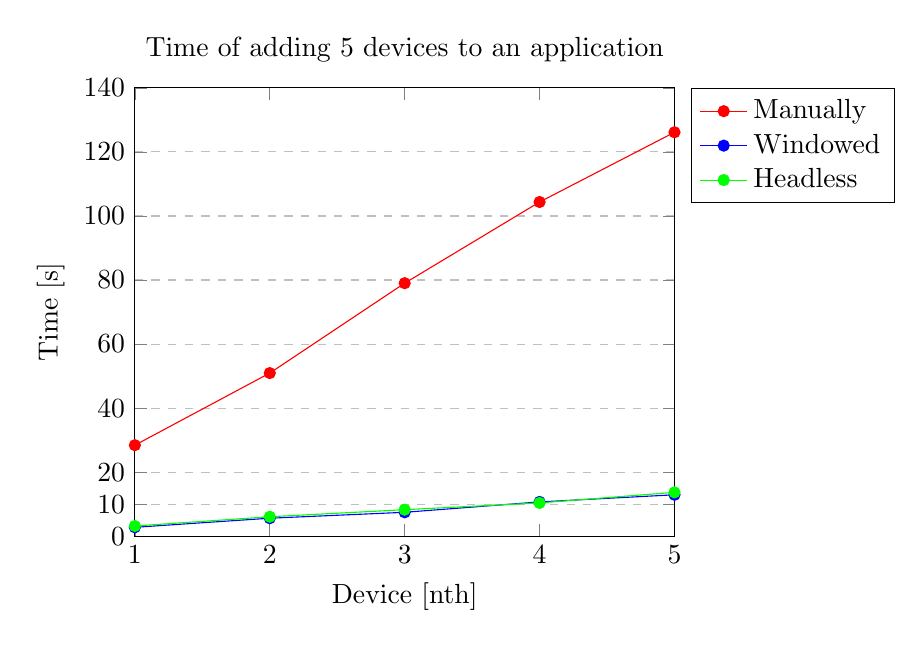
\begin{tikzpicture}
\begin{axis}[
    title={Time of adding 5 devices to an application},
    xlabel={Device [nth]},
    ylabel={Time [s]},
    xmin=1, xmax=5,
    ymin=0, ymax=140,
    xtick={1,2,3,4,5},
    ytick={0,10,20,40,60,80,100,120,140},
    legend pos=outer north east,
    legend cell align=left,
    ymajorgrids=true,
    grid style=dashed,
]

\addplot[
    color=red,
    mark=*,
    ]
    coordinates {
    (1,28.42)
    (2,50.94)
    (3,79.01)
    (4,104.36)
    (5,126.14)
    };
\addplot[
    color=blue,
    mark=*,
    ]
    coordinates{
    (1,2.776)
    (2,5.616)
    (3,7.463)
    (4,10.706)
    (5,12.929)
    };
\addplot[
    color=green,
    mark=*,
    ]
    coordinates{
    (1,3.176)
    (2,6.074)
    (3,8.274)
    (4,10.391)
    (5,13.692)
    };
    \legend{Manually, Windowed, Headless}
\end{axis}
\end{tikzpicture}

    \caption{Plot represents the results of testing the efficiency to add 5 devices to an application with three execution modes: manual, automated windowed mode and automated headless mode. Corresponding table to show data for each coordinate value is found from Table~\ref{tab:5_devices}}\label{fig:5_devices}
\end{figure}

\begin{figure}[H]
\centering
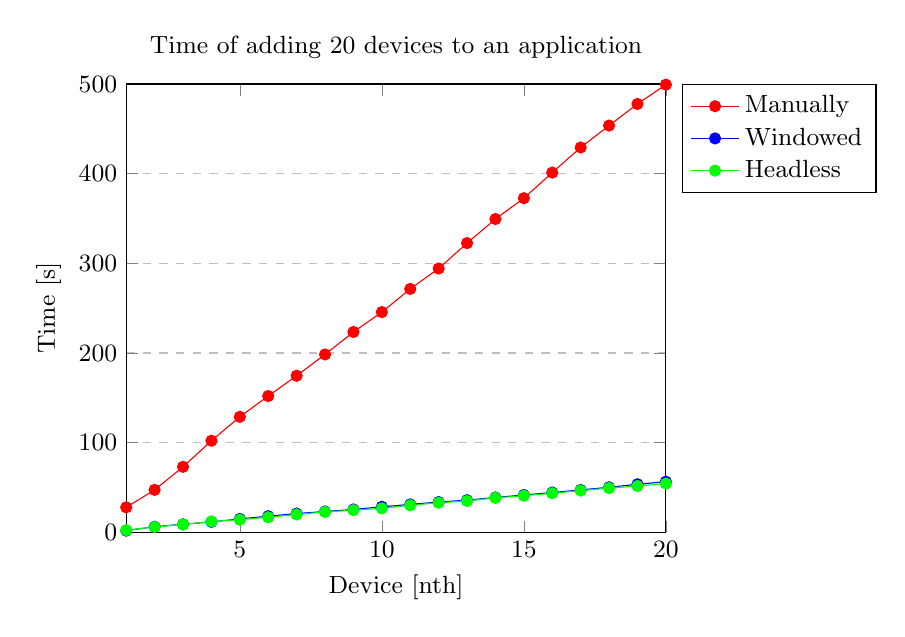
\begin{tikzpicture}
\begin{axis}[
    title={Time of adding 20 devices to an application},
    xlabel={Device [nth]},
    ylabel={Time [s]},
    xmin=1, xmax=20,
    ymin=0, ymax=500,
    xtick={0,5,10,15,20},
    ytick={0,100,200,300,400,500},
    legend pos=outer north east,
    legend cell align=left,
    ymajorgrids=true,
    grid style=dashed,
]

\addplot[
    color=red,
    mark=*,
    ]
    coordinates {
    (1,27.88)
    (2,47.36)
    (3,73.07)
    (4,102.17)
    (5,128.83)
    (6,152.03)
    (7,174.65)
    (8,198.41)
    (9,223.45)
    (10,245.63)
    (11,271.48)
    (12,294.25)
    (13,322.59)
    (14,349.44)
    (15,372.66)
    (16,401.25)
    (17,429.23)
    (18,453.67)
    (19,477.78)
    (20,499.28)
    };
\addplot[
    color=blue,
    mark=*,
    ]
    coordinates {
    (1,1.889)
    (2,6.244)
    (3,8.979)
    (4,11.591)
    (5,14.987)
    (6,18.008)
    (7,20.925)
    (8,23.241)
    (9,25.504)
    (10,28.466)
    (11,31.14)
    (12,33.822)
    (13,35.882)
    (14,38.861)
    (15,41.661)
    (16,44.417)
    (17,47.286)
    (18,50.244)
    (19,53.619)
    (20,56.474)
    };
\addplot[
    color=green,
    mark=*,
    ]
    coordinates {
    (1,2.413)
    (2,6.028)
    (3,8.763)
    (4,12.080)
    (5,14.112)
    (6,16.761)
    (7,19.961)
    (8,22.730)
    (9,24.710)
    (10,26.742)
    (11,30.158)
    (12,33.057)
    (13,35.023)
    (14,38.424)
    (15,40.858)
    (16,43.574)
    (17,46.574)
    (18,49.372)
    (19,51.672)
    (20,54.404)
    };
    \legend{Manually, Windowed, Headless}
    \small Plot showing the amount of time to add 20 devices.
\end{axis}
\end{tikzpicture}

    \caption{Plot represents the results of testing the efficiency to add 20 devices to an application with three execution modes: manual, automated windowed mode and automated headless mode.Corresponding table to show data for each coordinate value is found from Table~\ref{tab:20_devices}}\label{fig:20_devices}
\end{figure}

\begin{figure}[H]
\centering
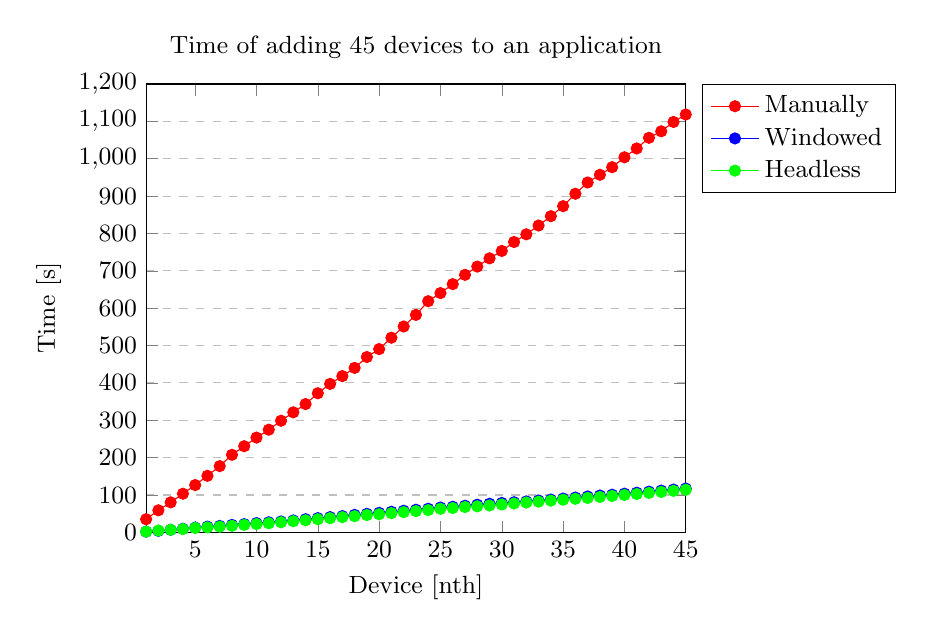
\begin{tikzpicture}
\begin{axis}[
    title={Time of adding 45 devices to an application},
    xlabel={Device [nth]},
    ylabel={Time [s]},
    xmin=1, xmax=45,
    ymin=0, ymax=1200,
    xtick={0,5,10,15,20,25,30,35,40,45},
    ytick={0,100,200,300,400,500,600,700,800,900,1000,1100,1200},
    legend pos=outer north east,
    legend cell align=left,
    ymajorgrids=true,
    grid style=dashed,
]

\addplot[
    color=red,
    mark=*,
    ]
    coordinates {
    (1,35.15)
    (2,59.01)
    (3,80.32)
    (4,103.42)
    (5,126.60)
    (6,151.33)
    (7,177.22)
    (8,207.59)
    (9,230.60)
    (10,253.61)
    (11,274.75)
    (12,298.70)
    (13,321.28)
    (14,343.35)
    (15,372.32)
    (16,397.39)
    (17,418.24)
    (18,440.21)
    (19,469.28)
    (20,490.53)
    (21,521.04)
    (22,551.04)
    (23,582.11)
    (24,618.71)
    (25,640.46)
    (26,664.43)
    (27,689.26)
    (28,711.40)
    (29,733.45)
    (30,753.23)
    (31,777.15)
    (32,797.72)
    (33,821.30)
    (34,846.26)
    (35,873.10)
    (36,906.32)
    (37,936.40)
    (38,957.09)
    (39,977.44)
    (40,1003.96)
    (41,1027.56)
    (42,1056.00)
    (43,1073.48)
    (44,1098.45)
    (45,1118.44)
    };
\addplot[
    color=blue,
    mark=*,
    ]
    coordinates {
    (1,1.915)
    (2,4.041)
    (3,6.777)
    (4,9.584)
    (5,12.646)
    (6,15.298)
    (7,17.269)
    (8,19.895)
    (9,21.986)
    (10,24.673)
    (11,26.902)
    (12,29.104)
    (13,31.922)
    (14,35.189)
    (15,37.995)
    (16,40.729)
    (17,43.367)
    (18,46.807)
    (19,49.507)
    (20,52.167)
    (21,55.02)
    (22,57.709)
    (23,60.466)
    (24,63.079)
    (25,66.391)
    (26,68.453)
    (27,71.064)
    (28,73.917)
    (29,76.447)
    (30,78.653)
    (31,80.53)
    (32,82.813)
    (33,85.196)
    (34,87.703)
    (35,90.392)
    (36,93.141)
    (37,96.044)
    (38,98.565)
    (39,100.655)
    (40,103.475)
    (41,106.123)
    (42,108.887)
    (43,111.672)
    (44,114.399)
    (45,117.309)
    };
\addplot[
    color=green,
    mark=*,
    ]
    coordinates {
    (1,1.954)
    (2,4.799)
    (3,6.93)
    (4,8.948)
    (5,11.764)
    (6,13.348)
    (7,15.314)
    (8,17.514)
    (9,19.999)
    (10,22.13)
    (11,24.297)
    (12,26.963)
    (13,29.763)
    (14,32.296)
    (15,35.081)
    (16,37.829)
    (17,40.613)
    (18,43.279)
    (19,46.279)
    (20,48.477)
    (21,51.327)
    (22,54.111)
    (23,56.759)
    (24,59.424)
    (25,63.008)
    (26,65.024)
    (27,67.758)
    (28,69.624)
    (29,71.956)
    (30,74.589)
    (31,77.189)
    (32,79.888)
    (33,82.121)
    (34,84.853)
    (35,87.352)
    (36,89.786)
    (37,92.118)
    (38,94.701)
    (39,97.401)
    (40,99.932)
    (41,102.536)
    (42,105.499)
    (43,108.149)
    (44,111.165)
    (45,113.998)};
    \legend{Manually, Windowed, Headless}
    \small Plot showing the amount of time to add 45 devices.
\end{axis}
\end{tikzpicture}
    \caption{Plot represents the results of testing the efficiency to add 45 devices to an application with three execution modes: manual, automated windowed mode and automated headless mode.Corresponding table to show data for each coordinate value is found from Table~\ref{tab:45_devices}}\label{fig:45_devices}
\end{figure}

\clearpage

\section{Faced difficulties}
The challenges that were faced during the project consisted of different kind of problems.
The most common ones would be trying to find errors that were faced during the testing of the features.
Most difficult ones to spot relating to that turned out to be the ones where syntax errors were occurring in the Robot Framework script, and incorrect amount of whitespace in different keywords.

The LORIX One gateway also provided some extra obstacles.
During testing, the web-interface started to refuse the connection and testing needed to be paused.
In the beginning this was handled by rebooting the server and it fixed the problem.
The reason for this was not found.

Later on there was a new problem, when the feature of deleting a selected device from the decided application was being tested.
This feature had functioned correctly earlier and no changes were made to the Robot Framework script. 
The problem was noticed when the gateway had been rebooted and the testing was continued for that feature.
The problem was that when a device is being deleted from an application, after clicking the delete button the user is to be expecting a confirmation message.
Instead the server showed a pop-up error message on the bottom left page as seen in Figure~\ref{fig:error_when_confirming_device_deleting}.

\begin{figure}[ht]
  \centering
  {\includegraphics[width=\textwidth]{illustration/error_when_confirming_device_deleting.PNG}}
  \caption{Error message about refused connection to the Redis server that is run by the ChirpStack \gls{os}}
  \label{fig:error_when_confirming_device_deleting}
\end{figure}

Further investigation through ChirpStack forum resulted to find people with similar problem when using the same gateway \cite{chirpstack_forum:redis_error}.
Later on in the discussion, a user proposed a possible solution that can be found in an opened issue on GitHub \cite{github:redis_issue}.
A collaborator in the GitHub project had made changes to the \path{redis.conf} file in the ChirpStack \gls{os} to fix the issue.
That same fix was used in this project to outrun the problem and it got solved.

During the last few test runs the connection to the web-interface was corrupted again, the issue being that while the user got logged in, no applications were visible in the server and therefor they were not accessible either.
The first hand solution, that worked, was to disconnect the gateway for overnight and turn it on again.
After that the issue never came back, so there was no further investigation.

Overall these server obstacles slowed down the project implementation with several days.
Further investigation should be considered if the problems continue.
This might require to take some actions, like updating the software versions, or even to change the hardware that is used, as most of the challenges were reflected to the use of the LORIX One gateway.
The consideration should also take in account the load the gateway has been under during the testing.
The implementation is most likely not used as heavily in such short-term , as it has during the testing phases.


\section{Maintainability}
 Upon the beginning of the project it was decided that the automation was to be implemented by using Robot Framework.
 The hardware was decided to be the same that Metropolia University of Applied Sciences already use and it was delivered by them.

The implementation relies completely on the web-interface of the ChirpStack Application server.
The variables are created by using the selectors of the elements in the web-interface and they are hard-coded to the variables.py file.
If any changes to the web-interface is made, it might lead to breaking the Robot Framework script, or at least to a large amount of redefinition of the variables and possibly the keywords as well.

The LORIX One gateway only supports the ChirpStack up to the version 3, and all the implementation is also based to that version.
The most latest version of the ChirpStack is currently version 4.
If the gateway hardware, or the ChirpStack version is to be updated, it might make the implementation incompatible.

\section{Improvement ideas}

The implementation is currently made with the assumption that there is less than 100 applications listed, meaning they would be visible on a single page when the rows per page selection is set to 100.
And same default base is also used with the devices that are added to a single application.
If the amount of those applications or devices is greater than 100, the ones that are crossing the limit are shown in the next page,  and therefore aren't processed as part of the list.
Currently the rows per page amount is set in the suite setup and the selected row amount is automatically set to it in every list type in the web-interface.
This should be changed in the next possible update to make the implementation more reliable.

The running time of the Robot Framework script, when multiple devices are added, could possibly be further reduced by handling all the message pop-ups that the device creation triggers.
Currently it verifies that there is no message about duplicate device, but on a successful device creation there is a device created message as well. 
This message leads to extra waiting time as the script recognizes it to one of the pop-ups and starts the timeout which delays the running time.
This issue could be solved for example by closing the device created pop-up, whenever it is triggered.

Robocorp announced the joining to Sema4.ai on the end of January \cite{robocorp:sema4.ai}.
In the following month they published that they are focusing to develop the automation further only in Python language.
The implementation is currently using the Excel.Files library of RPA Framework to interact with the Excel files, using Robot Framework.
The new direction Robocorp is taking with the code focused automation means that the existing Robot Framework based libraries are being spared, but no new updates or issue fixes are done in regards to them.
In practise this affects the upcoming development, which should be considered if this project is to be further developed.

During the research about the ChirpStack Application server, it was found out that ChirpStack provides \gls{grpc} and \gls{rest}ful APIs \cite{chirpstack:applicationServer}.
ChirpStack stood down from using \gls{rest} API from the version 4 onwards.
With this in mind, it should be considered if the script is to be updated, that if it should be implemented by using the API provided with the \gls{grpc} instead of the current automation of the web-interface.
This would provide a list of more reliable commands to use for handling the tasks in the server.

\clearpage

Using the \gls{grpc} framework requires a decision about what programming language to use with it.
The \gls{grpc} officially supports 10 different languages, like C++, Python, Java, and Node.js to name a few examples, but there are also some community-based implementations available.

Even if the implementation would start to use \gls{grpc}, Robot Framework can still be the framework to be used.
Robot Framework supports extending through Python libraries and ChirpStack also supplies a Python \gls{sdk} for the \gls{grpc}.
With these complabilities in mind, Python could be considered as a strong candidate from the programming language options to use with the \gls{grpc}.



\clearpage %force the next chapter to start on a new page. Keep that as the last line of your chapter!